
\begin{center}
\Huge
	Sinusrelationerne
\end{center}

\section*{Sinusrelationerne}
\stepcounter{section}



Vi kan bruge arealformlen til at sige noget om forholdene mellem vinklerne og sidelængderne i vilkårlige trekanter. Disse forhold kaldes for \textit{sinusrelationerne.}

\begin{figure}[H]
	\centering
	\begin{tikzpicture}
		\draw[color = olive, thick] (0,0) -- (5,0) node[midway, anchor = north] {$b$};
		\draw[color = olive, thick] (0,0) -- (4,3) node[midway, anchor = south east] {$c$};
		\draw[color = olive, thick] (5,0) -- (4,3) node[midway, anchor = west] {$a$};
		\node[color = olive, anchor = east] at (0,0) {$A$};
		\node[color = olive, anchor = west] at (5,0) {$C$};
		\node[color = olive, anchor = south] at (4,3) {$B$};
	\end{tikzpicture}
	\caption{Vilkårlig trekant $\triangle ABC$}
	\label{fig:vilkårlig}
\end{figure}

\begin{setn}[Sinusrelationerne]
	\label{setn:sinusrelation}
	For vilkårlige trekanter $\triangle ABC$ som den på Figur \ref{fig:vilkårlig} gælder der, at 
	\begin{align}
		\label{eq:sin1}
		\frac{\sin(\angle A)}{a} = \frac{\sin(\angle B)}{b} = \frac{\sin(\angle C)}{c}.
	\end{align}
	Vi kan tilsvarende skrive sinusrelationernes som
	\begin{align}
		\label{eq:sin2}
		\frac{a}{\sin(\angle A)} = \frac{b}{\sin(\angle B)} = \frac{c}{\sin(\angle C)}.
	\end{align}
\end{setn}
\begin{proof}
	Opgave
\end{proof}

For at se, hvordan sinusrelationerne kan anvendes, ses der på et eksempel.
\begin{exa}
	En trekant er givet ved følgende.
	\begin{center}
		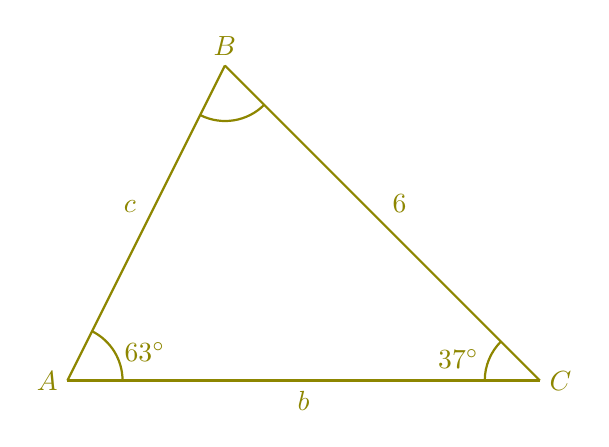
\begin{tikzpicture}
		%A
		\pgfmathsetmacro{\ax}{0}
		\pgfmathsetmacro{\ay}{0}
		%B
		\pgfmathsetmacro{\bx}{2}
		\pgfmathsetmacro{\by}{4}
		%C
		\pgfmathsetmacro{\cx}{6}
		\pgfmathsetmacro{\cy}{0}
		%arc radius
		\pgfmathsetmacro{\arclen}{0.7}
		%c
		\draw[color = olive, thick] (\ax,\ay) -- (\bx,\by) node[midway, anchor = south east] {$c$};
		%b
		\draw[color = olive, thick] (\ax,\ay) -- (\cx,\cy) node[midway, anchor = north] {$b$};
		%a
		\draw[color = olive, thick] (\bx,\by) -- (\cx,\cy) node[midway, anchor = south west] {$6$};
	%	Vinkel A		
		\draw[color = olive, thick] (\ax + \arclen,0) arc (0:63.43:\arclen) 
		node[midway, anchor = west] {$63^{\circ}$};
	%	Vinkel B
		\draw[color = olive, thick] (1.69,3.37) arc (180 + 63.43:180 + 63.43 + 71.57:\arclen)
		 node[midway, anchor = south east] {};
	%	Vinkel C
		\draw[color = olive, thick] (\cx - \arclen,0) arc (180:180 - 45:\arclen)
		 node[midway, anchor = east] {$37^\circ$};
		 %Nodes
		 \node[color = olive, anchor = east] at (\ax,\ay) {$A$};
		 \node[color = olive, anchor = south] at (\bx,\by) {$B$};
		 \node[color = olive, anchor = west] at (\cx,\cy) {$C$};
		\end{tikzpicture}
	\end{center}
	Vi kender $\angle A = 63^\circ$, $\angle C = 37^\circ$ og $a = 6$. Vi kan indsætte dette i 
	sinusrelationerne og får
	\begin{align*}
		\frac{\sin(\angle A)}{a} = \frac{\sin(\angle C)}{c} \Leftrightarrow 
		\frac{\sin(67^\circ)}{6} = \frac{\sin(37^\circ)}{c}
	\end{align*}
	Vi aflæser $\sin(63^\circ) = 0.9$ og $\sin(37^\circ) = 0.6$
	 i Tabel \ref{tab:cossintan} med én decimal.
	Dette indsættes i ligningen og vi får
	\begin{align*}
		\frac{\sin(67^\circ)}{6} = \frac{\sin(37^\circ)}{c} &\Leftrightarrow	
		\frac{0.9}{6} = \frac{0.6}{c} \\
		&\Leftrightarrow	 c = \frac{6\cdot 0.6}{0.9} = \frac{3.6}{0.9} = 4,
	\end{align*}
	og derfor er $c = 4$. 
\end{exa} 

Når vi skal bestemme sidelængder med sinusrelationerne, er det nemmest at bruge \eqref{eq:sin2}, og når vi tilsvarende skal bestemme vinkler med sinusrelationerne, er det nemmest at bruge \eqref{eq:sin1}.

\newpage


\begin{table}[H]
	\centering
	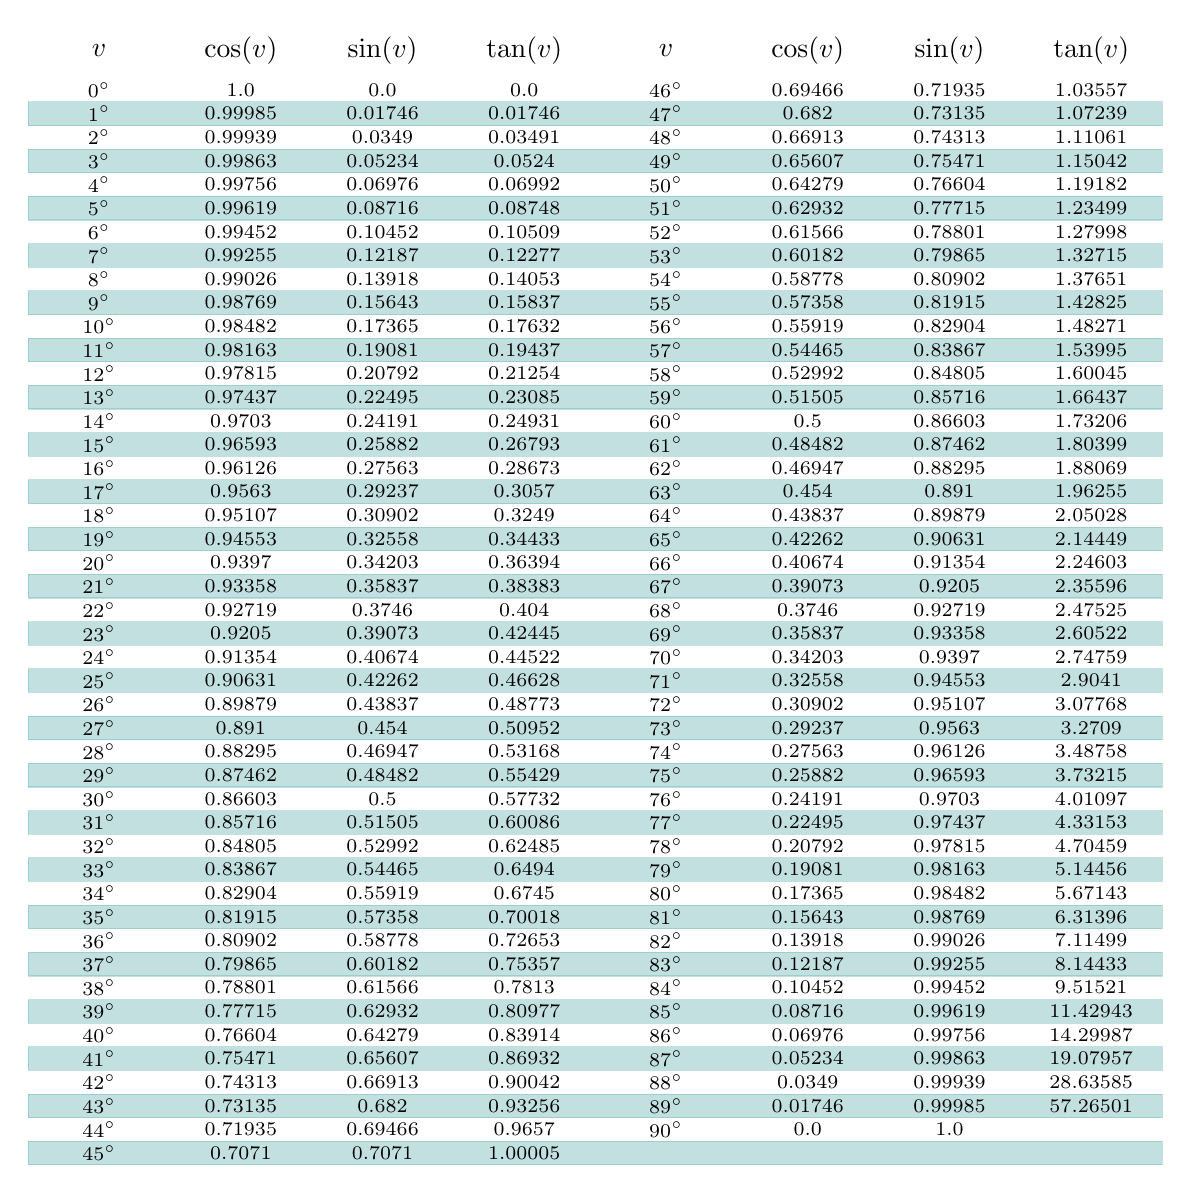
\begin{tikzpicture}
	\node at (0,0) {$v$};
	\node at (2*0.9,0) {$\cos(v)$};
	\node at (4*0.9,0) {$\sin(v)$};
	\node at (6*0.9,0) {$\tan(v)$};
	\node at (8*0.9,0) {$v$};
	\node at (10*0.9,0) {$\cos(v)$};
	\node at (12*0.9,0) {$\sin(v)$};
	\node at (14*0.9,0) {$\tan(v)$};
	\scriptsize
	%Colors
	\foreach \i in {0,...,22}{
		\filldraw[color = teal!60, opacity = 0.4] (-0.9,-0.5-0.3+0.15-\i*0.3*2) rectangle
		 (14*0.9 + 0.9,-0.5-0.3-0.15-\i*0.3*2);
	}
	\foreach \i in {0,...,45}{
		%Macros for evaluating
		\pgfmathsetmacro{\cval}{cos(\i)}
		\pgfmathsetmacro{\sval}{sin(\i)}
		\pgfmathsetmacro{\tval}{tan(\i)}
		%First columns of values
		\node at (0,-0.5-\i*0.3) {$\i^{\circ}$};
		\node at (2*0.9,-0.5-\i*0.3) { \cval };
		\node at (4*0.9,-0.5-\i*0.3) { \sval };
		\node at (6*0.9,-0.5-\i*0.3) { \tval };
	}
	\foreach \i in {46,...,89}{
		%Macros
		\pgfmathsetmacro{\cval}{cos(\i)}
		\pgfmathsetmacro{\sval}{sin(\i)}
		\pgfmathsetmacro{\tval}{tan(\i)}
		%Second column
		\node at (8*0.9,-0.5-\i*0.3 + 46*0.3) {$\i^{\circ}$};
		\node at (10*0.9,-0.5-\i*0.3 + 46*0.3) { \cval };
		\node at (12*0.9,-0.5-\i*0.3 + 46*0.3) { \sval };
		\node at (14*0.9,-0.5-\i*0.3 + 46*0.3) { \tval };
	}
		\pgfmathsetmacro{\cval}{cos(90)}
		\pgfmathsetmacro{\sval}{sin(90)}
		\node at (8*0.9,-0.5-90*0.3 + 46*0.3) {$90^{\circ}$};
		\node at (10*0.9,-0.5-90*0.3 + 46*0.3) { \cval };
		\node at (12*0.9,-0.5-90*0.3 + 46*0.3) { \sval };
	\end{tikzpicture}
	\caption{Tabel over udvalgte værdier for $\cos$, $\sin$ og $\tan$.}
	\label{tab:cossintan}
\end{table}

\newpage

\subsection*{Opgave 1}
Til de følgende to delopgaver skal du bruge Tabel \ref{tab:cossintan}, hvor du afrunder til to decimaler.
\begin{enumerate}[label=\roman*)]
	\item Bestem sidelængden $a$ i den første trekant.
	\item Bestem sidelængden $c$ i den anden trekant. 
\begin{center}
	\begin{minipage}{0.45\textwidth}
		\centering
		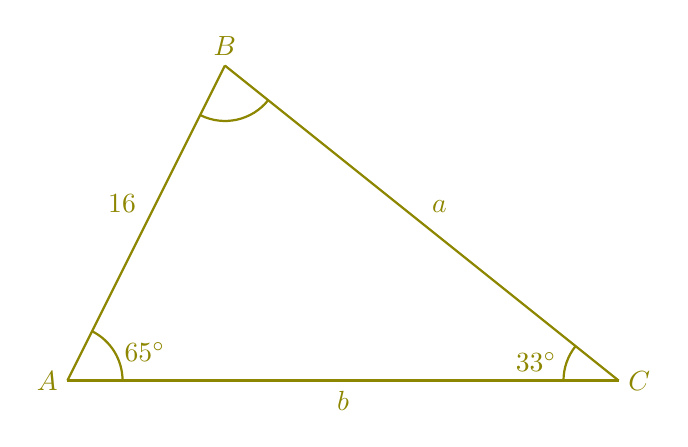
\begin{tikzpicture}
		%A
		\pgfmathsetmacro{\ax}{0}
		\pgfmathsetmacro{\ay}{0}
		%B
		\pgfmathsetmacro{\bx}{2}
		\pgfmathsetmacro{\by}{4}
		%C
		\pgfmathsetmacro{\cx}{7}
		\pgfmathsetmacro{\cy}{0}
		%arc radius
		\pgfmathsetmacro{\arclen}{0.7}
		%c
		\draw[color = olive, thick] (\ax,\ay) -- (\bx,\by) node[midway, anchor = south east] {$16$};
		%b
		\draw[color = olive, thick] (\ax,\ay) -- (\cx,\cy) node[midway, anchor = north] {$b$};
		%a
		\draw[color = olive, thick] (\bx,\by) -- (\cx,\cy) node[midway, anchor = south west] {$a$};
	%	Vinkel A		
		\draw[color = olive, thick] (\arclen,0) arc (0:63.43:\arclen) 
		node[midway, anchor = west] {$65^\circ$};
	%	Vinkel B
		\draw[color = olive, thick] (1.69,3.37) arc (180 + 63.53:180 + 63.43 + 77.91:\arclen)
		 node[midway, anchor = south] {};
	%	Vinkel C
		\draw[color = olive, thick] (\cx - \arclen,0) arc (180:180 - 38.66:\arclen)
		 node[midway, anchor = east] {$33^\circ$};
		 %Nodes
		 \node[color = olive, anchor = east] at (\ax,\ay) {$A$};
		 \node[color = olive, anchor = south] at (\bx,\by) {$B$};
		 \node[color = olive, anchor = west] at (\cx,\cy) {$C$};
		\end{tikzpicture}
	\end{minipage}
	\begin{minipage}{0.45\textwidth}
		\centering
		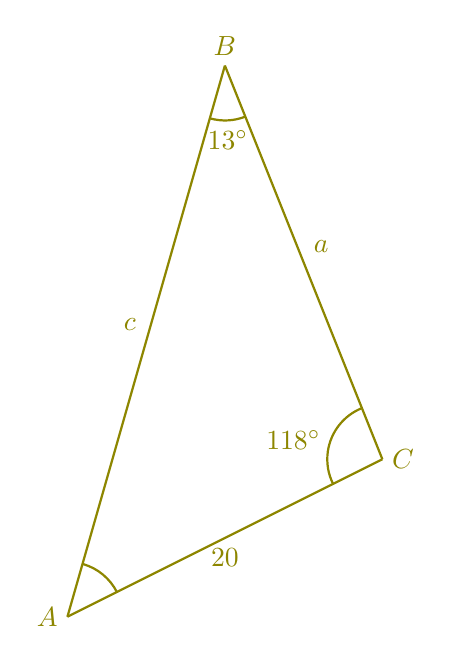
\begin{tikzpicture}
		%A
		\pgfmathsetmacro{\ax}{0}
		\pgfmathsetmacro{\ay}{0}
		%B
		\pgfmathsetmacro{\bx}{2}
		\pgfmathsetmacro{\by}{7}
		%C
		\pgfmathsetmacro{\cx}{4}
		\pgfmathsetmacro{\cy}{2}
		%arc radius
		\pgfmathsetmacro{\arclen}{0.7}
		%c
		\draw[color = olive, thick] (\ax,\ay) -- (\bx,\by) node[midway, anchor = south east] {$c$};
		%b
		\draw[color = olive, thick] (\ax,\ay) -- (\cx,\cy) node[midway, anchor = north] {$20$};
		%a
		\draw[color = olive, thick] (\bx,\by) -- (\cx,\cy) node[midway, anchor = south west] {$a$};
	%	Vinkel A		
		\draw[color = olive, thick] (0.63,0.31) arc (26.57:47.49+26.57:\arclen) 
		node[midway, anchor = south west] {};
	%	Vinkel B
		\draw[color = olive, thick] (1.81,6.33) arc (180 + 74.05:180+74.05+37.75:\arclen)
		 node[midway, anchor = north] {$13^{\circ}$};
	%	Vinkel C
		\draw[color = olive, thick] (3.74,2.65) arc (111.8:111.8+94.76:\arclen)
		 node[midway, anchor = east] {$118^\circ$};
		 %Nodes
		 \node[color = olive, anchor = east] at (\ax,\ay) {$A$};
		 \node[color = olive, anchor = south] at (\bx,\by) {$B$};
		 \node[color = olive, anchor = west] at (\cx,\cy) {$C$};
		\end{tikzpicture}
	\end{minipage}
\end{center}
\end{enumerate}

\subsection*{Opgave 2}
Til de følgende to delopgaver skal du bruge Tabel \ref{tab:cossintan}, hvor du afrunder til to decimaler.
\begin{enumerate}[label=\roman*)]
	\item Bestem vinklen $\angle A$ i den første trekant.
	\item Bestem vinklen $\angle B$ i den anden trekant. Husk, at den er stump. 
\end{enumerate}
\begin{center}
	\begin{minipage}{0.40\textwidth}
		\centering
		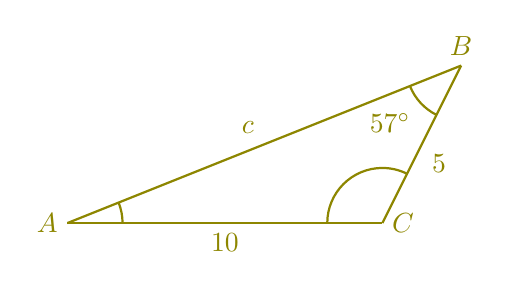
\begin{tikzpicture}
		%A
		\pgfmathsetmacro{\ax}{0}
		\pgfmathsetmacro{\ay}{0}
		%B
		\pgfmathsetmacro{\bx}{5}
		\pgfmathsetmacro{\by}{2}
		%C
		\pgfmathsetmacro{\cx}{4}
		\pgfmathsetmacro{\cy}{0}
		%arc radius
		\pgfmathsetmacro{\arclen}{0.7}
		%c
		\draw[color = olive, thick] (\ax,\ay) -- (\bx,\by) node[midway, anchor = south east] {$c$};
		%b
		\draw[color = olive, thick] (\ax,\ay) -- (\cx,\cy) node[midway, anchor = north] {$10$};
		%a
		\draw[color = olive, thick] (\bx,\by) -- (\cx,\cy) node[midway, anchor = north west] {$5$};
	%	Vinkel A		
		\draw[color = olive, thick] (\arclen,0) arc (0:21.8:\arclen) 
		node[midway, anchor = west] {};
	%	Vinkel B
		\draw[color = olive, thick] (4.35,1.74) arc (180 + 21.8:180 + 21.8 + 41.68:\arclen)
		 node[midway, anchor = north east] {$57^\circ$};
	%	Vinkel C
		\draw[color = olive, thick] (\cx - \arclen,0) arc (180:180 - 116.57:\arclen)
		 node[midway, anchor = east] {};
		 %Nodes
		 \node[color = olive, anchor = east] at (\ax,\ay) {$A$};
		 \node[color = olive, anchor = south] at (\bx,\by) {$B$};
		 \node[color = olive, anchor = west] at (\cx,\cy) {$C$};
		\end{tikzpicture}
	\end{minipage}
	\begin{minipage}{0.55\textwidth}
		\centering
		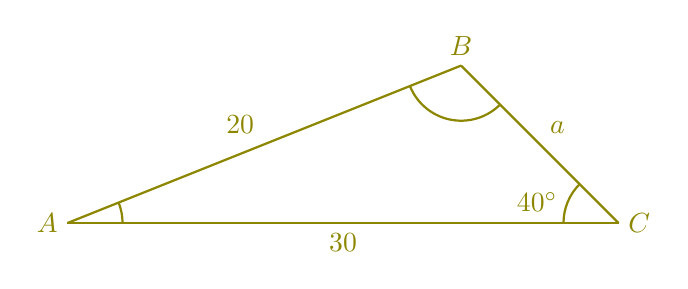
\begin{tikzpicture}
		%A
		\pgfmathsetmacro{\ax}{0}
		\pgfmathsetmacro{\ay}{0}
		%B
		\pgfmathsetmacro{\bx}{5}
		\pgfmathsetmacro{\by}{2}
		%C
		\pgfmathsetmacro{\cx}{7}
		\pgfmathsetmacro{\cy}{0}
		%arc radius
		\pgfmathsetmacro{\arclen}{0.7}
		%c
		\draw[color = olive, thick] (\ax,\ay) -- (\bx,\by) node[midway, anchor = south east] {$20$};
		%b
		\draw[color = olive, thick] (\ax,\ay) -- (\cx,\cy) node[midway, anchor = north] {$30$};
		%a
		\draw[color = olive, thick] (\bx,\by) -- (\cx,\cy) node[midway, anchor = south west] {$a$};
	%	Vinkel A		
		\draw[color = olive, thick] (\arclen,0) arc (0:21.8:\arclen) 
		node[midway, anchor = west] {};
	%	Vinkel B
		\draw[color = olive, thick] (4.35,1.74) arc (180 + 21.8:180 + 21.8 + 113.2:\arclen)
		 node[midway, anchor = north east] {};
	%	Vinkel C
		\draw[color = olive, thick] (\cx - \arclen,0) arc (180:180 - 45:\arclen)
		 node[midway, anchor = east] {$40^\circ$};
		 %Nodes
		 \node[color = olive, anchor = east] at (\ax,\ay) {$A$};
		 \node[color = olive, anchor = south] at (\bx,\by) {$B$};
		 \node[color = olive, anchor = west] at (\cx,\cy) {$C$};
		\end{tikzpicture}
	\end{minipage}
\end{center}

\subsection*{Opgave 3 (med hjælpemidler)}
En trekant $\triangle ABC$ opfylder, at $\angle A = 29^\circ$, $\angle B = 55^\circ$ og $b = 3$.
\begin{enumerate}[label=\roman*)]
	\item Tegn en skitse af $\triangle ABC$. 
	\item Bestem sidelængden $a$.
\end{enumerate}

\subsection*{Opgave 4 (med hjælpemidler)}
En trekant $\triangle ABC$ opfylder, at $\angle B = 130^\circ$, $b = 50$ og $c = 10$.
\begin{enumerate}[label=\roman*)	]
	\item Tegn en skitse af $\triangle ABC$. 
	\item Bestem vinklen $\angle C$. 
\end{enumerate}

\subsection*{Opgave 5}
En trekant $\triangle ABC$ har $a = 48$, $b = 12$ og $\angle B = 8^\circ$.
\begin{enumerate}[label=\roman*)]
	\item Bestem $\angle A$, hvis det oplyses, at $\angle A$ er stump. Brug Tabel \ref{tab:cossintan} med to 
	decimaler. 
\end{enumerate}

\subsection*{Opgave 6}
En trekant $\triangle ABC$ opfylder, at $\angle C = 166^\circ$, $\angle B = 7^\circ$ og $b = 6$.
\begin{enumerate}[label=\roman*)]
	\item Bestem sidelængden $c$. Brug Tabel \ref{tab:cossintan} med to 
	decimaler. 
\end{enumerate}

\subsection*{Opgave 7}

En trekant $\triangle ABC$ opfylder, at $\angle B = 30^\circ$ og $\angle A = 90^\circ$.
\begin{enumerate}[label=\roman*)]
	\item Hvor meget længere er sidelængden $a$ end sidelængden $b$? Brug evt. Tabel \ref{tab:cossintan}.
\end{enumerate} 

\subsection*{Opgave 8}
Vi skal bevise Sætning \ref{setn:sinusrelation}.
\begin{enumerate}[label=\roman*)]
	\item Udnyt at arealet $M$ for en vilkårlig trekant $\triangle ABC$ kan skrives på følgende tre måder
	\begin{align*}
		M = \frac{1}{2}ab\sin(\angle C) = \frac{1}{2}ac\sin(\angle B) = \frac{1}{2} bc\sin(\angle A)
	\end{align*}
	og dividér hele ligheden med $\frac{1}{2}abc$.
	\item Forkort udtrykket.
\end{enumerate}



\subsection*{Opgave 9 (fra sidst)}
Til de følgende to delopgaver skal du bruge Tabel \ref{tab:cossintan}, hvor du afrunder til én decimal.
\begin{enumerate}[label=\roman*)]
	\item Bestem sidelængden $c$ i den første trekant.
	\item Bestem sidelængden $a$ i den anden trekant. 
\end{enumerate}
\begin{center}
	\begin{minipage}{0.45\textwidth}
		\centering
		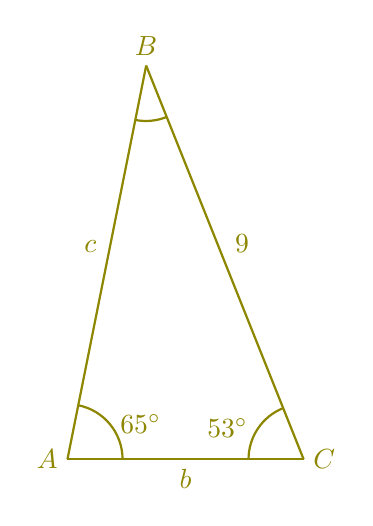
\begin{tikzpicture}
		%A
		\pgfmathsetmacro{\ax}{0}
		\pgfmathsetmacro{\ay}{0}
		%B
		\pgfmathsetmacro{\bx}{1}
		\pgfmathsetmacro{\by}{5}
		%C
		\pgfmathsetmacro{\cx}{3}
		\pgfmathsetmacro{\cy}{0}
		%arc radius
		\pgfmathsetmacro{\arclen}{0.7}
		%c
		\draw[color = olive, thick] (\ax,\ay) -- (\bx,\by) node[midway, anchor = south east] {$c$};
		%b
		\draw[color = olive, thick] (\ax,\ay) -- (\cx,\cy) node[midway, anchor = north] {$b$};
		%a
		\draw[color = olive, thick] (\bx,\by) -- (\cx,\cy) node[midway, anchor = south west] {$9$};
	%	Vinkel A		
		\draw[color = olive, thick] (\arclen,0) arc (0:78.68:\arclen) 
		node[midway, anchor = west] {$65^\circ$};
	%	Vinkel B
		\draw[color = olive, thick] (0.86,4.31) arc (180 + 78.69:180 + 78.69 + 33.11:\arclen)
		 node[midway, anchor = south] {};
	%	Vinkel C
		\draw[color = olive, thick] (\cx - \arclen,0) arc (180:180 - 68.20:\arclen)
		 node[midway, anchor = east] {$53^\circ$};
		 %Nodes
		 \node[color = olive, anchor = east] at (\ax,\ay) {$A$};
		 \node[color = olive, anchor = south] at (\bx,\by) {$B$};
		 \node[color = olive, anchor = west] at (\cx,\cy) {$C$};
		\end{tikzpicture}
	\end{minipage}
		\begin{minipage}{0.45\textwidth}
		\centering
		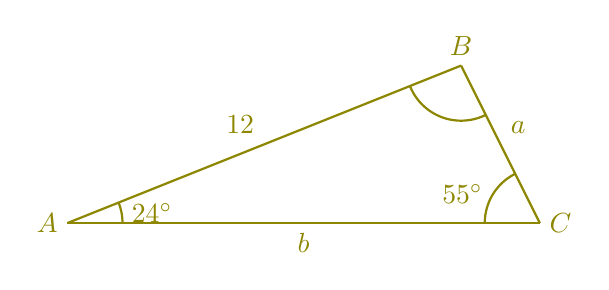
\begin{tikzpicture}
		%A
		\pgfmathsetmacro{\ax}{0}
		\pgfmathsetmacro{\ay}{0}
		%B
		\pgfmathsetmacro{\bx}{5}
		\pgfmathsetmacro{\by}{2}
		%C
		\pgfmathsetmacro{\cx}{6}
		\pgfmathsetmacro{\cy}{0}
		%arc radius
		\pgfmathsetmacro{\arclen}{0.7}
		%c
		\draw[color = olive, thick] (\ax,\ay) -- (\bx,\by) node[midway, anchor = south east] {$12$};
		%b
		\draw[color = olive, thick] (\ax,\ay) -- (\cx,\cy) node[midway, anchor = north] {$b$};
		%a
		\draw[color = olive, thick] (\bx,\by) -- (\cx,\cy) node[midway, anchor = south west] {$a$};
	%	Vinkel A		
		\draw[color = olive, thick] (\arclen,0) arc (0:21.8:\arclen) 
		node[midway, anchor = west] {$24^\circ$};
	%	Vinkel B
		\draw[color = olive, thick] (4.35,1.74) arc (180 + 21.8:180 + 21.8 + 94.76:\arclen)
		 node[midway, anchor = south] {};
	%	Vinkel C
		\draw[color = olive, thick] (\cx - \arclen,0) arc (180:180 - 63.43:\arclen)
		 node[midway, anchor = east] {$55^\circ$};
		 %Nodes
		 \node[color = olive, anchor = east] at (\ax,\ay) {$A$};
		 \node[color = olive, anchor = south] at (\bx,\by) {$B$};
		 \node[color = olive, anchor = west] at (\cx,\cy) {$C$};
		\end{tikzpicture}
	\end{minipage}
\end{center}
\subsection*{Opgave 10 (fra sidst)}
Til de følgende to delopgaver skal du bruge Tabel \ref{tab:cossintan}, hvor du afrunder til én decimal.
\begin{enumerate}[label=\roman*)]
	\item Bestem $\angle B$ i den første trekant.
	\item Bestem $\angle C$ i den anden trekant. 
\end{enumerate}

\begin{center}
	\begin{minipage}{0.45\textwidth}
		\centering
		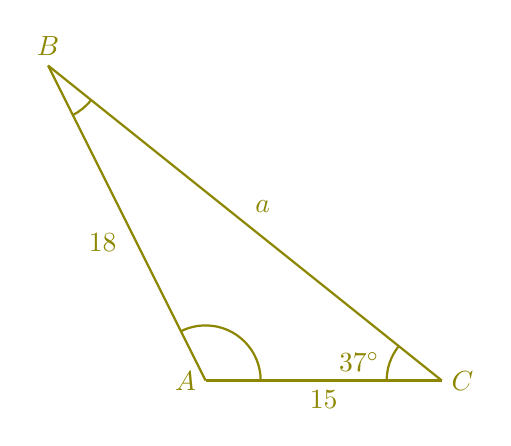
\begin{tikzpicture}
		%A
		\pgfmathsetmacro{\ax}{2}
		\pgfmathsetmacro{\ay}{0}
		%B
		\pgfmathsetmacro{\bx}{0}
		\pgfmathsetmacro{\by}{4}
		%C
		\pgfmathsetmacro{\cx}{5}
		\pgfmathsetmacro{\cy}{0}
		%arc radius
		\pgfmathsetmacro{\arclen}{0.7}
		%c
		\draw[color = olive, thick] (\ax,\ay) -- (\bx,\by) node[midway, anchor = north east] {$18$};
		%b
		\draw[color = olive, thick] (\ax,\ay) -- (\cx,\cy) node[midway, anchor = north] {$15$};
		%a
		\draw[color = olive, thick] (\bx,\by) -- (\cx,\cy) node[midway, anchor = south west] {$a$};
	%	Vinkel A		
		\draw[color = olive, thick] (\ax + \arclen,0) arc (0:116.57:\arclen) 
		node[midway, anchor = west] {};
	%	Vinkel B
		\draw[color = olive, thick] (0.31,3.37) arc (180 + 116.57:180 + 116.57 + 24.78:\arclen)
		 node[midway, anchor = south east] {};
	%	Vinkel C
		\draw[color = olive, thick] (\cx - \arclen,0) arc (180:180 - 38.66:\arclen)
		 node[midway, anchor = east] {$37^\circ$};
		 %Nodes
		 \node[color = olive, anchor = east] at (\ax,\ay) {$A$};
		 \node[color = olive, anchor = south] at (\bx,\by) {$B$};
		 \node[color = olive, anchor = west] at (\cx,\cy) {$C$};
		\end{tikzpicture}
	\end{minipage}
		\begin{minipage}{0.45\textwidth}
		\centering
		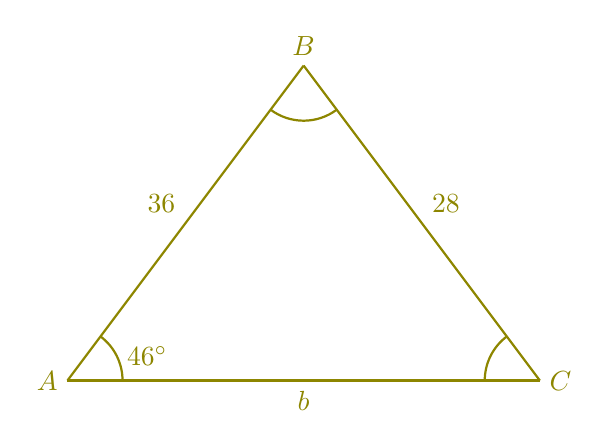
\begin{tikzpicture}
		%A
		\pgfmathsetmacro{\ax}{0}
		\pgfmathsetmacro{\ay}{0}
		%B
		\pgfmathsetmacro{\bx}{3}
		\pgfmathsetmacro{\by}{4}
		%C
		\pgfmathsetmacro{\cx}{6}
		\pgfmathsetmacro{\cy}{0}
		%arc radius
		\pgfmathsetmacro{\arclen}{0.7}
		%c
		\draw[color = olive, thick] (\ax,\ay) -- (\bx,\by) node[midway, anchor = south east] {$36$};
		%b
		\draw[color = olive, thick] (\ax,\ay) -- (\cx,\cy) node[midway, anchor = north] {$b$};
		%a
		\draw[color = olive, thick] (\bx,\by) -- (\cx,\cy) node[midway, anchor = south west] {$28$};
	%	Vinkel A		
		\draw[color = olive, thick] (\ax + \arclen,0) arc (0:53.13:\arclen) 
		node[midway, anchor = west] {$46^{\circ}$};
	%	Vinkel B
		\draw[color = olive, thick] (2.58,3.44) arc (180 + 53.13:180 + 53.13 + 73.74:\arclen)
		 node[midway, anchor = south east] {};
	%	Vinkel C
		\draw[color = olive, thick] (\cx - \arclen,0) arc (180:180 - 53.13:\arclen)
		 node[midway, anchor = east] {};
		 %Nodes
		 \node[color = olive, anchor = east] at (\ax,\ay) {$A$};
		 \node[color = olive, anchor = south] at (\bx,\by) {$B$};
		 \node[color = olive, anchor = west] at (\cx,\cy) {$C$};
		\end{tikzpicture}
	\end{minipage}
\end{center}